\documentclass[fleqn,10pt]{wlscirep}
\usepackage[utf8]{inputenc}
\usepackage[T1]{fontenc}
\usepackage{lineno}
\usepackage{multirow}
\usepackage{makecell}
\usepackage{color,soul}
\linenumbers

\title{Inflation of test accuracy due to data leakage in deep learning-based classification of OCT images}

\author[1,2,*]{Iulian Emil Tampu}
\author[1,2,3]{Anders Eklund}
\author[1,2]{Neda Haj-Hosseini}
\affil[1]{Department of Biomedical Engineering , Linköping University, 581 85 Linköping,  Sweden}
\affil[2]{Center for Medical Image Science and Visualization , Linköping University, 581 83 Linköping,  Sweden}
\affil[3]{Division of Statistics \& Machine Learning, Department of Computer and Information Science, Linköping University, 581 83 Linköping,  Sweden}

\affil[*]{corresponding author: Iulian Emil Tampu (iulian.emil.tampu@liu.se)}

% \affil[$\dag$]{these authors contributed equally to this work}


\begin{abstract}
In the application of deep learning on optical coherence tomography (OCT) data, it is common to train classification networks using 2D images originating from volumetric data. Given the micrometer resolution of OCT systems, consecutive images are often very similar in both visible structures and noise. Thus, an inappropriate data split can result in overlap between the training and testing sets, with a large portion of the literature overlooking this aspect. In this study, the effect of improper dataset splitting on model evaluation is demonstrated for three classification tasks using three OCT open-access datasets extensively used in the literature, Kermany’s and Srinivas ophthalmology datasets and AIIMS breast tissue dataset. Our results show that the classification Matthew correlation coefficient is inflated by 7.5 up to 21.7 percentage units for models tested on a dataset with improper splitting, highlighting the considerable effect of dataset handling on model evaluation. This study intends to raise awareness on the importance of dataset splitting for research on deep learning using OCT data and volumetric data in general. 
\end{abstract}
\begin{document}

\flushbottom
\maketitle
%  Click the title above to edit the author information and abstract

\thispagestyle{empty}

\section*{Introduction}
The evaluation of deep learning models, and in general machine learning methods, aims at providing an unbiased description of model performance. Given a pool of data suitable for studying a hypothesis (e.g. classification, regression or segmentation), different splits of the data are commonly created for model training, model hyper-parameter tuning (validation set) and model assessment (testing set). This translates to having a part of the data used to fit model parameters and tune model hyperparameters, and another set to assess model generalization on unseen data \cite{xu2018splitting}. Disregarding the choice of having separate validation and testing splits \cite{kuhn2013applied}, the strategy used to generate the testing set from the original pool of data can have a large impact on the assessment of the model's final performance. Several studies have investigated the effect of the relative size between training, validation and/or testing sets \cite{xu2018splitting, guyon1997scaling} on model performance, as well as how training and validation sets can be used via resampling techniques, such as cross-validation, during model training \cite{xu2018splitting, refaeilzadeh2009cross}. More importantly, it is widely accepted that no overlap should exist between the samples used for model fitting and hyperparameter tuning, and those belonging to the testing set. If overlap is present, the model performance will be biased and uninformative with respect to the generalization capabilities of the model to new samples. However, although trivial, when implementing data splitting strategies the overlap between training and testing sets can be easily overlooked. This is especially true for 3D medical image data, as 2D methods are often applied to individual slices given the limited amount of memory of graphics hardware. A proper splitting must therefore be done on the volume or subject level and not on slice level.

Nowadays, machine learning methods, especially convolutional neural networks (CNNs) and deep learning algorithms, are widely used in research to analyze medical image data. A plethora of publications describe CNN implementations on a variety of both 2D and 3D medical data \cite{litjens2017survey, ker2017deep, anwar2018medical}. Reliable evaluation of such methods is paramount since this informs the research community on the models’ performance, allows meaningful comparison between methods, and to a greater extent indicates which research questions might be worth further investigation. To this regard, many medical image analysis challenges were established that aim at providing an unbiased platform for the evaluation and ranking of different methods on a common and standard testing dataset. In a review, Maier-Hein et al. \cite{maier2018rankings} have collected the majority of the available medical image competitions and analyzed the reliability of such challenges. Despite the many limitations discovered, including missing information regarding how the ground truth was obtained, the authors emphasized the importance of these challenges and their contribution towards a more transparent and reliable evaluation of deep learning methods for medical image applications.

However, not all implementations can be evaluated through dedicated challenges. Thus, when such third-party evaluation platforms are not available, it is the responsibility of the researchers performing the investigation to evaluate their \mbox{method thoroughly}. As for the case of many of the reviewed medical image analysis challenges \cite{maier2018rankings}, one aspect that is sometimes missing or not well described is how the testing dataset is generated from the original pool of data. Moreover, there are also examples where the preparation of the testing dataset is described, but its overlap with the training set was not considered \cite{wang2019deep, butola2020deep, irmak2021multi, sadad2021brain, yagis2021effect}, undermining the reproducibility of the study as well as the reliability of the reported results. This is specifically more common in those applications where, due to hardware limitations or model design choices, the data from one subject (or acquisition) is used to obtain multiple dimensionally-smaller samples used for model training and testing. An example of such a scenario is the slicing of a 3D volume into 2D images. In these cases, the overlap between training and testing sets results from having 2D images from the same subject (or acquisition) belonging to both sets.
\begin{figure}[t]
\centering
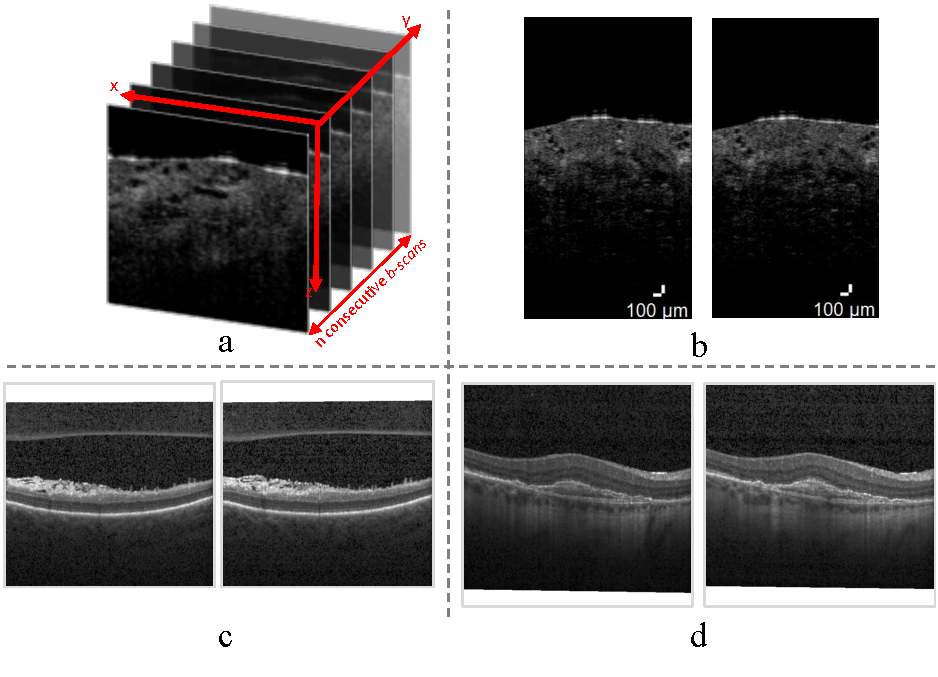
\includegraphics[width=420pt]{OCT_inflation_intro_dataset_v1.pdf}
\caption{Schematic of an OCT volume with examples of consecutive slices (\textit{b-scans}) from the three open-access OCT datasets used in this study. (a) pictures the consecutive 2D \textit{b-scans} rendering a 3D OCT volume. Here an example from the AIIMS dataset \cite{butola2019volumetric} is used for illustrative purposes. In (b) the consecutive \textit{b-scans} separated by $\sim$18 micrometers are examples of healthy breast tissue (Patient 15, volume 0046, slices 0075 and 0076) from the AIIMS dataset \cite{butola2019volumetric}. (c) shows consecutive images of retina affected by choroidal neovascularization (CNV 81630-33 and 81630-34) from the Kermany’s OCT2017 dataset \cite{kermany2018large}.  (d) images of age-related macular degeneration (AMD) from Srinivas dataset (AMD2 046 and 047).
Note that the \textit{b-scans} from both Kermany’s and Srinivas' dataset are given with data augmentation applied.}
\label{fig:introduction_1}
\end{figure}

Focusing on deep-learning applications for optical coherence tomography (OCT), the pool of data used for model training and testing commonly originates from volumetric acquisitions of the same samples under investigation. Depending on the acquisition set-up, volumes are usually acquired with micrometer resolution in the x, y and z directions in a restricted field of view, with tissue structures that are alike and affected by similar noise, resulting in consecutive slices having a high similarity. Figure \ref{fig:introduction_1} shows a schematic of an OCT volume along with examples of two consecutive slices from OCT volumes from three open-access datasets \cite{butola2019volumetric, kermany2018large}. 

The majority of the reviewed literature implementing deep learning on OCT data used 2D images from scanned volumes, where two methods were commonly used to split the pool of image data into training and testing: \textit{per-image} or \textit{per-volume/subject} splitting. 
In the \textit{per-volume/subject} splitting approach,  the random selection of data for the testing set is done on the volumes (or subjects) ensuring that images from one volume (or subject) belong to either one of the training or testing sets. It is important to notice that even a \textit{per-volume} split might not be enough to avoid overlap between the training and testing set. In fact, if multiple volumes are acquired from the same tissue region, the tissue structures will be very similar among the volumes. In these scenarios, a \textit{per-subject} split is more appropriate. Overall, assuming that volumes are acquired from different tissue regions, splitting the dataset \textit{per-volume} or \textit{per-subject} (here called \textit{per-volume/subject}) ensures that overlap between training and testing is not present.
On the other hand in the \textit{per-image} approach, 2D images belonging to the same volume are considered independent. Thus, the testing set is created by random selection from the pool of images without considering that images from the same volume (or subject) might end up in both the training and testing sets.  \hl{Even if this approach clearly results in overlap between the the testing and training sets,  a number of reviewed studies as well as one of the most downloaded open-access OCT dataset employed a \textit{per-image} split.} 

%On the other hand in the \textit{per-volume/subject} splitting approach, the random selection of data for the testing set is done on the volumes (or subjects) ensuring that images from one volume (or subject) belong to either one of the training or testing sets. It is important to notice that even a \textit{per-volume} split might not be enough to avoid overlap between the training and testing set. In fact, if multiple volumes are acquired from the same tissue region, the tissue structures will be very similar among the volumes. In these scenarios, a \textit{per-subject} split is more appropriate. Overall, assuming that volumes are acquired from different tissue regions, splitting the dataset \textit{per-volume} or \textit{per-subject} (here called \textit{per-volume/subject}) ensures that overlap between training and testing is not present.

Thus, the aim of this study is to demonstrate the effect of improper dataset splitting (\textit{per-image}) on classification accuracy using three open-access OCT datasets, Kermany’s OCT2017 \cite{kermany2018large},  AIIMS \cite{butola2019volumetric} and Srinivas \cite{srinivasan2014fully}. These were selected among the other open-access datasets for several reasons: (1) they are examples of OCT medical images belonging to different medical disciplines (ophthalmology and breast oncology) and showing different tissue structures and textures, (2) they are used in literature to evaluate deep learning-based classification of OCT images, with Kermany’s dataset \cite{kermany2018large} extensively used for developing deep learning methods in ophthalmology (over 14,500 downloads) \cite{Retinalkaggle}, and (3) the datasets are provided in two different ways, per-subject for the AIIMS and Srinivas dataset, and already split for Kermany’s datasets. The latter is an important aspect to consider since many of the studies using Kermany’s dataset overlooked the overlap between the training and the testing data. 

\section*{Results}
LightOCT model classification performance on the three datasets and for the different dataset split strategies, is summarized in Table \ref{tab:results_1}, with results presented as mean$\pm$standard deviation (mean$\pm$std) over the ten repeated five-fold cross validation.  In addition, Figure \ref{fig:results_1}a shows in details the MCC distribution as box plots.  For all datasets, the \textit{per-image} split strategy results in a higher model performance compared to the \textit{per-volume/subject} strategy.  In particular, looking at the results on Kermany’s dataset, the mean MCC dropped by 7.9 percentage units when shifting from a \textit{per-image} strategy to a \textit{per-volume/subject} one.  An even larger decrease in performance is seen when comparing the model trained on the \textit{per-volume/subject} with the one trained on the \textit{original split},  which contains overlapping testing and training images,  with mean MCC and AUC reduced by 28.3 and 7 percentage units,  respectively.  A similar trend can be seen for the both the AIIMS and Srinivas datasets,  where the model trained on the dataset using \textit{per-image} strategy had a mean MCC higher by 7.5 and 21.7 percentage units, respectively,  compared to the one trained on a \textit{per-volume/subject} split.  \\
Results on the random label experiment are presented in Figure \ref{fig:results_1}b for all datasets and dataset split strategies.  These show that the mean MCC is close to zero for all the tests performed, describing the random classification of the model.
%\begin{table}[ht]
%\centering
%\caption{\label{tab:results_1}LightOCT model performance on Kermany’s \cite{kermany2018large} and AIIMS \cite{butola2019volumetric} datasets with training, validation and testing sets split using different strategies. Performance metrics are reported as mean$\pm$standard deviation (mean$\pm$std) over the models trained through 5-fold cross validation, and classes. }
%\renewcommand{\arraystretch}{1.5}
%\begin{tabular}{|c|c|c|c|c|c|c|}
%\hline
%\textit{Dataset} & \textit{Split strategy} &  \makecell{ \textit{Accuracy} \\ \textit{(mean$\pm$std)}} &  \makecell{\textit{Precision} \\ \textit{(mean$\pm$std)}} &  \makecell{\textit{Recall} \\ \textit{(mean$\pm$std)}} &  \makecell{\textit{F1-score} \\ \textit{(mean$\pm$std)}} &  \makecell{\textit{AUC} \\ \textit{(mean$\pm$std)}} \\
%\hline\hline
%\multirow{4}{*}{\makecell{Kermany's \cite{kermany2018large} \\ dataset} } &  \makecell{Results from \cite{butola2020deep} \\ using \textit{original split}} & $\sim$0.96 & / & 0.95 & / & / \\
%\cline{2-7}
%& \textit{original split} & 0.926 & 0.981 & 0.926 & 0.925 & 0.993 \\
%\cline{2-7}
%& \textit{per-image split} & 0.793$\pm$0.011 &  0.893$\pm$0.007 & 0.793$\pm$0.011 & 0.789$\pm$0.012 & 0.955$\pm$0.003 \\
%\cline{2-7}
%&  \makecell{\textit{per-volume/subject} \\ \textit{split}} & 0.667$\pm$0.017 & 0.764$\pm$0.013 & 0.667$\pm$0.017 & 0.655$\pm$0.022 & 0.896$\pm$0.007 \\
%\hline
%\hline
%\multirow{3}{*}{\makecell{AIIMS \cite{butola2019volumetric} \\ dataset} } &  \makecell{Results from \cite{butola2020deep} \\ using \textit{per-image split}} & 0.988 & 0.993 & 0.986 & 0.989 & 0.996 \\
%\cline{2-7}
%& \textit{per-image split} & 0.987$\pm$0.003 & 0.997$\pm$00.004 & 0.987$\pm$0.003 & 0.987$\pm$0.003 & 0.997$\pm$0.004 \\
%\cline{2-7}
%&  \makecell{\textit{per-volume/subject} \\ \textit{split}} & 0.948$\pm$0.007 & 0.966$\pm$0.005 & 0.948$\pm$0.007 & 0.948$\pm$0.007 & 0.971$\pm$0.003\\
%\hline
%\end{tabular}
%\end{table}

\begin{table}[ht]
\centering
\caption{\label{tab:results_1}LightOCT model performance on Kermany’s \cite{kermany2018large},  AIIMS \cite{butola2019volumetric} and Srinivas \cite{srinivasan2014fully} datasets with training, validation and testing sets split using different strategies. Performance metrics are reported as mean$\pm$standard deviation (mean$\pm$std) over the models trained through the ten repeated five-fold cross validation and classes. }
\renewcommand{\arraystretch}{1.5}
\begin{tabular}{|c|c|c|c|c|c|c|c|}
\hline
\textit{Dataset} & \textit{Split strategy} &  \makecell{ \small{\textit{MCC} [-1,1]} \\ \textit{(mean$\pm$std)}} &  \makecell{ \small{\textit{AUC} [0,1]} \\ \textit{(mean$\pm$std)}} &  \makecell{\small{\textit{F1-score} [0,1]} \\ \textit{(mean$\pm$std)}} &  \makecell{\small{\textit{Accuracy} [0,1]} \\ \textit{(mean$\pm$std)}} &  \makecell{\small{\textit{Precision} [0,1]} \\ \textit{(mean$\pm$std)}} & \makecell{\small{\textit{Recall} [0,1]}\\ \textit{(mean$\pm$std)}} \\
\hline\hline
\multirow{4}{*}{\makecell{Kermany's \cite{kermany2018large} \\ dataset} } &  \makecell{Results from \cite{butola2020deep} \\ using \textit{original split}} & \small{/} & \small{/} & \small{/} &  \small{$\sim$0.96} & \small{/} & \small{0.945} \\
\cline{2-8}
& \textit{original split} & \small{0,906}  & \small{0,992}  & \small{0,927}  & \small{0,928} & \small{0,979} & \small{0,928} \\
\cline{2-8}
& \textit{per-image split} &  \small{0,702$\pm$0,015}  & \small{0,953$\pm$0,003}  & \small{0,758$\pm$0,015}  & \small{0,765$\pm$0,013}  & \small{0,891$\pm$0,006}  & \small{0,765$\pm$0,013}  \\
\cline{2-8}
&  \makecell{\textit{per-volume/subject} \\ \textit{split}} &  \small{0,623$\pm$0,015}  & \small{0,915$\pm$0,006}  & \small{0,681$\pm$0,018}  & \small{0,694$\pm$0,014}  & \small{0,804$\pm$0,011}  & \small{0,694$\pm$0,014} \\
\hline
\hline
\multirow{3}{*}{\makecell{AIIMS \cite{butola2019volumetric} \\ dataset} } &  \makecell{Results from \cite{butola2020deep} \\ using \textit{per-image split}} & \small{/} & \small{0.996} & \small{0.989} & \small{0.988} & \small{0.993} & \small{0.986}  \\
\cline{2-8}
& \textit{per-image split} & \small{0,982$\pm$0,006}  & \small{0,999$\pm$0,001}  & \small{0,991$\pm$0,003}  & \small{0,9911$\pm$0,003}  & \small{0,999$\pm$0,001}  & \small{0,991$\pm$0,003} \\
\cline{2-8}
&  \makecell{\textit{per-volume/subject} \\ \textit{split}} & \small{0,907$\pm$0,106}  & \small{0,996$\pm$0,007}  & \small{0,949$\pm$0,064}  & \small{0,950$\pm$0,061}  & \small{0,995$\pm$0,009}  & \small{0,950$\pm$0,061} \\
\hline
\hline
\multirow{3}{*}{\makecell{Srinivas \cite{srinivasan2014fully} \\ dataset} } &  \makecell{Results from \cite{butola2020deep} \\ using \textit{per-image split}} & \small{/} & \small{/} & \small{/} & \small{>0.96} & \small{/} & \small{0. 988}\\
\cline{2-8}
& \textit{per-image split} &  \small{0,881$\pm$0,016}  & \small{0,987$\pm$0,003}  & \small{0,920$\pm$0,011}  & \small{0,920$\pm$0,011}  & \small{0,976$\pm$0,006}  & \small{0,920$\pm$0,011} \\
\cline{2-8}
&  \makecell{\textit{per-volume/subject} \\ \textit{split}} & \small{0,447$\pm$0,109}  & \small{0,828$\pm$0,054}  & \small{0,607$\pm$0,0712}  & \small{0,617$\pm$0,071}  & \small{0,720$\pm$0,079}  & \small{0,617$\pm$0,071}  \\
\hline
\end{tabular}
\end{table}

\begin{figure}[t]
\centering
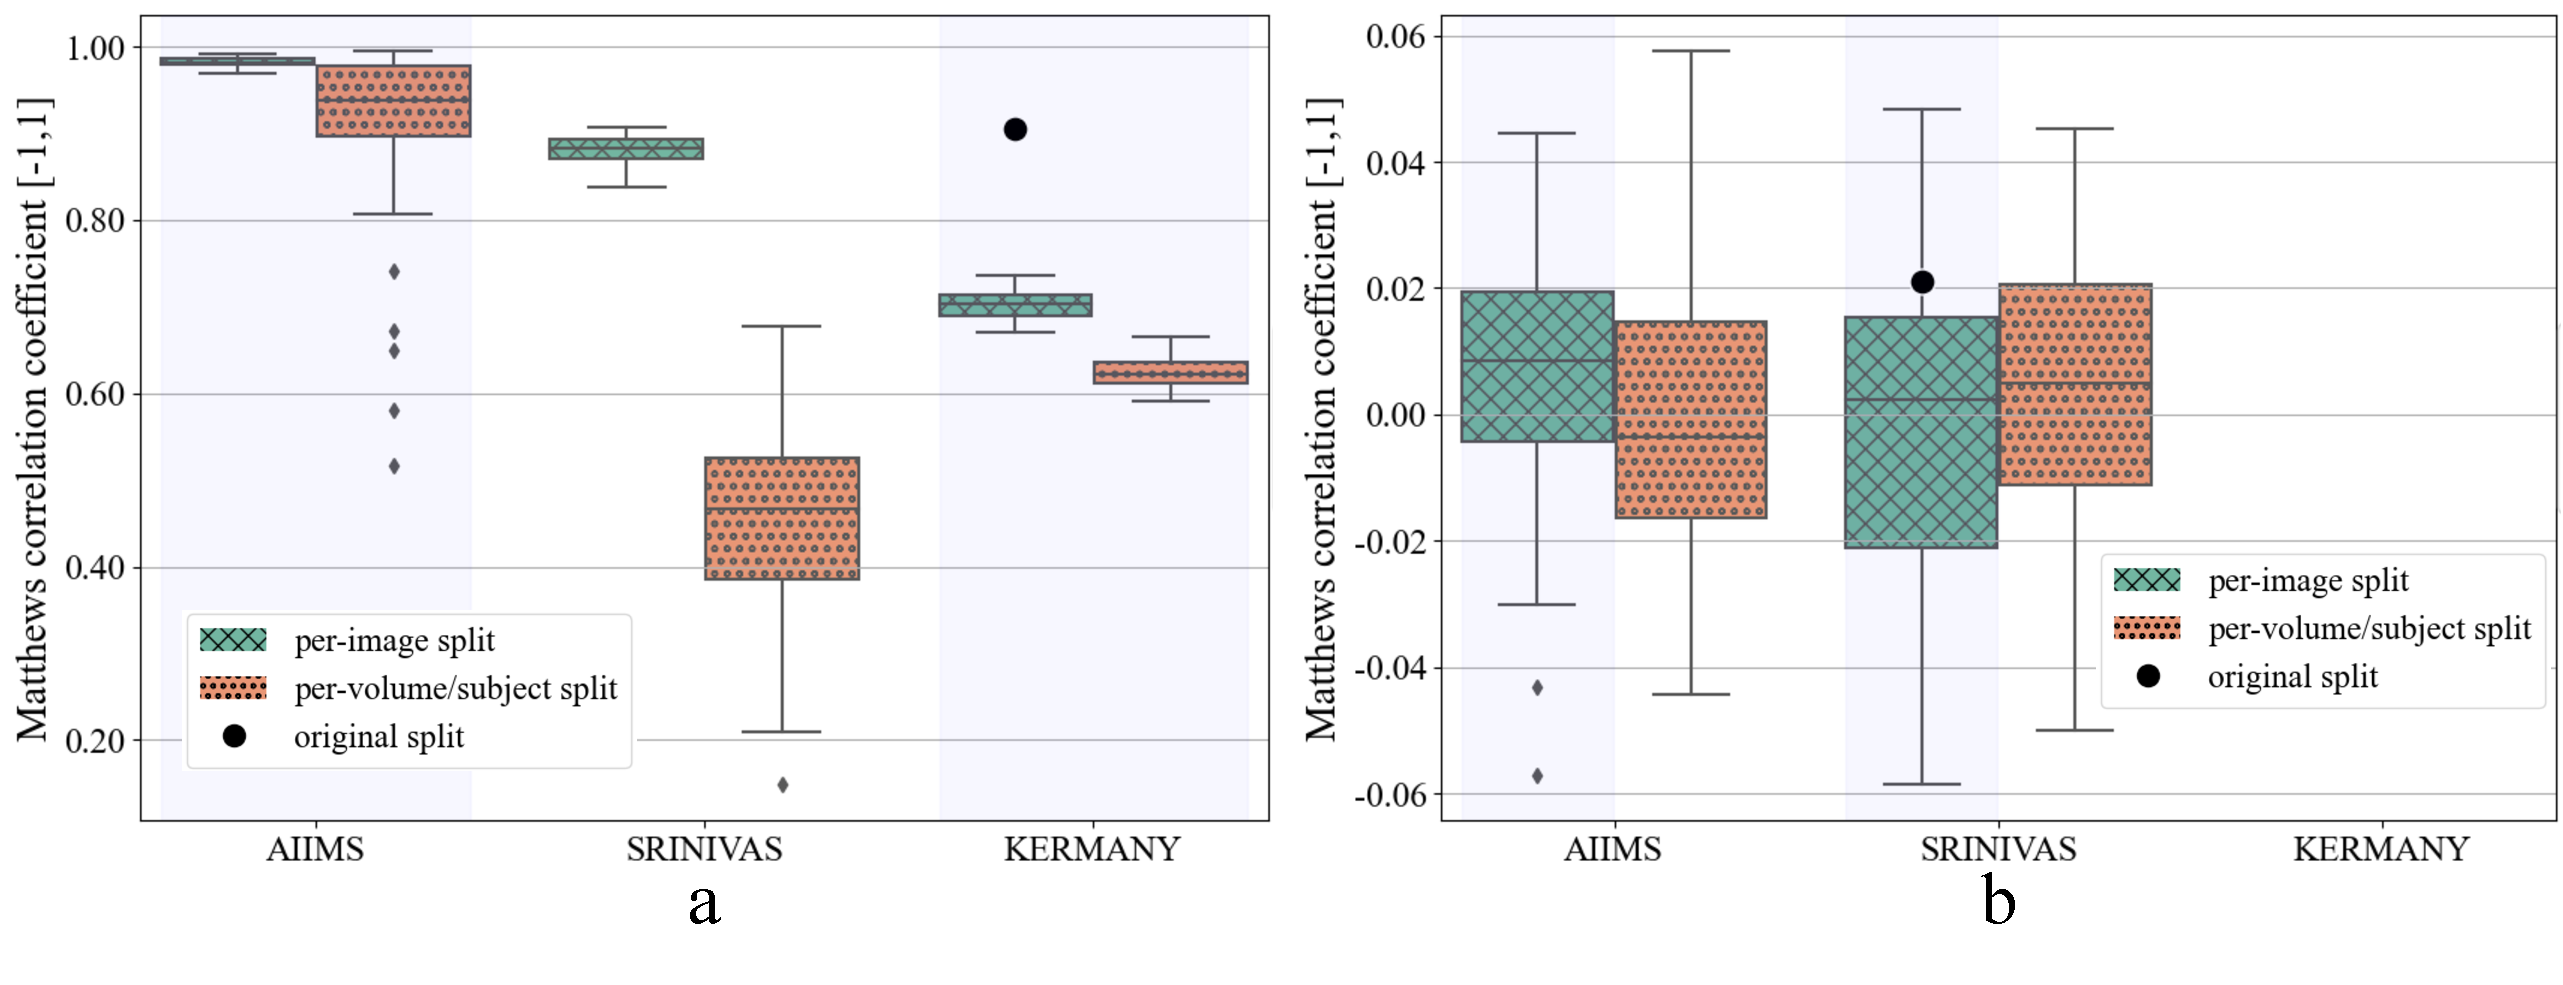
\includegraphics[width=500pt]{OCT_inflation_results_1_v2.pdf}
\caption{Comparison between Matthews correlation coefficient comparison for LightOCT model trained on different dataset split strategies.  In (a) the results with each sample having the correct label, whereas in (b) the results from the random bales experiment. For both (a) and (b) each box plot summarise the test MCC for the 50 models trained through a ten repeated five-fold cross validation.  Results are presented for all the three datasets with the \textit{per-image} split strategy shown in striped-green and \textit{per-volume/subject} split strategy in dotted-orange. For Kermany's dataset, the result of the models trained on the original split is shown as full-black circle. \hl{Figure b needs to include the results from Kermany's trainings}}
%\caption{Macro-average ROC curves showing a comparison between LightOCT model performance trained on (a) Kermany’s \cite{kermany2018large} and (b) AIIMS \cite{butola2019volumetric} dataset with training, validation and test sets created using different split strategies. The performance metrics (AUC, F1-score and accuracy) for the \textit{per-image} and \textit{per-volume/subject} results were obtained as an ensemble by majority voting of the five models trained through cross validation. In (a), results on the original, \textit{per-image} and \textit{per-volume/subject} splits are shown in solid blue, dashed yellow and dash-dotted green. In (b), model performance on the \textit{per-image} and \textit{per-volume/subject} split strategies are shown in solid blue and dashed yellow, respectively.}
\label{fig:results_1}
\end{figure}
\section*{Discussion}
Dataset split should be carefully designed to avoid overlap between training and testing sets. Table \ref{tab:discussion_1} summarizes several studies on deep learning applications for OCT data, specifying the described data split strategy. All the works using the \textit{original split} from Kermany’s dataset or a \textit{per-image} split strategy reported accuracies >95\%. Obtained results are in accordance with the reported values on Kermany’s original split, where the difference in performance can be attributed to the optimization of the LightOCT model. Interestingly, Table \ref{tab:discussion_1} also shows that studies using multiple datasets and reporting different split strategies for each dataset \cite{butola2020deep,kamran2019optic, thomas2021novel}, show as high accuracy on the \mbox{\textit{per-volume/subject}} split datasets as the one on the \textit{original split} or the \textit{per-image} split datasets. In the light of our results and the overlap found between the training and testing sets in Kermany’s \textit{original split}, it is reasonable to ask whether the high performances reported for the \textit{per-volume/subject} split datasets reflect the true high performance of the implemented methods, or are examples of inflated accuracy values due to data leakage between training and testing sets. 

\hl{Another source of data leakage, which was not investigated in this study but that could similarly inflate classification performance, is data augmentation.  In particular, an image could be augmented many time with its different augmented versions ending in the training and testing set.  This result in a data overlap similar to the one of a \textit{per-image} split strategy, where images with the same structures and noise properties are in both training and testing sets. The original split in Kermany dataset is provided with already augmented images. Overlap between training and testing with respect to data augmentation was not checked. }

In conclusion, the used dataset split strategy can have a substantial impact on the evaluation of deep learning models. In this paper it is demonstrated that, in OCT image classification applications specifically, a \textit{per-image} split strategy of the volumetric data adopted by a considerable number of studies, returns over-optimistic results on model performance and an inflation of test accuracy values, questioning the reliability of the assessments and hindering an objective comparison between research outcomes.  This problem has also been demonstrated in 3D magnetic resonance imaging studies \cite{yagis2021effect} and in digital pathology \cite{bussola2021ai}, where data leakage between the training and testing sets resulted in over-optimistic classification accuracy.Moreover, greater attention should be paid to the structure of datasets made available to the research community to avoid biasing the evaluation of different methods and undermining the usefulness of open-access datasets.  \hl{With the increase focus of research community in the implementation of deep learning methods for OCT image analysis, the presented results want to raise awareness on a trivial but overlooked problem that can spoil research efforts.}

\begin{table}[ht]
\centering
\caption{\label{tab:discussion_1} Summary of reviewed literature with focus on dataset split and reported test classification performance. Open-access datasets and the ones available upon request are marked by $^\ast$ and $^{\ast\ast}$, respectively. Dataset is not open-access if not specified. Datasets obtained from animal model samples are marked by $^\dagger$. The difference in performance between studies using the same datasets results from the different implemented methods.}
\renewcommand{\arraystretch}{1.5}
\begin{tabular}{|c|l|l|l|}
\hline
\textit{Ref.} & \textit{OCT dataset} & \textit{Data split strategy} & \textit{Model performance on testing set} \\
\hline\hline
\cite{wang2019deep} & \makecell[l]{Data from thyroid, parathyroid, fat \\ and muscle samples} & \textit{per-image} &  97.12\% accuracy \\
\hline
\cite{najeeb2018classification} & Ophthalmology \cite{kermany2018large}$^\ast$ & \textit{original split} & 95.55\% accuracy \\
\hline
\cite{chen2021classification} & Ophthalmology \cite{kermany2018large}$^\ast$ & \textit{original split} & 99.1\% accuracy \\
\hline
\cite{latha2021automated} & Ophthalmology \cite{kermany2018large}$^\ast$ & \textit{original split} & 98.7\% accuracy \\
\hline
\cite{latha2021automated} & Ophthalmology \cite{kermany2018large}$^\ast$ & \textit{original split} & 96.6\% accuracy \\
\hline
\cite{tsuji2020classification} & Ophthalmology \cite{kermany2018large}$^\ast$ & \textit{original split} & 99.6\% accuracy \\
\hline
\cite{kamran2019optic} & \makecell[l]{(1) Ophthalmology \cite{kermany2018large}$^\ast$ \\(2) Ophthalmology \cite{srinivasan2014fully}$^\ast$} & \makecell[l]{(1) \textit{original split}\\(2) \textit{per-volume/subject}} & \makecell[l]{(1) 99.80\% accuracy\\(2) 100\% accuracy} \\
\hline
\cite{athanasiou2019deep} & Coronary artery OCT & \textit{per-volume/subject} & 96.05\% accuracy \\
\hline
\cite{wang2021deep} & Kidney$^\dagger$ & \textit{per-volume/subject} & 82.6\% accuracy \\
\hline
\cite{gesperger2020improved} & Data from high and low grade brain tumors & \textit{per-volume/subject} & 97\% accuracy \\
\hline
\cite{saratxaga2021characterization} & Colon$^{\ast \ast, \dagger}$ & \textit{per-volume/subject} & 88.95\% accuracy on 2D images \\
\hline
\cite{singla2019automated} & Data from breast tissue & \textit{per-volume/subject} & 91.7\% specificity \\
\hline
\cite{chetoui2020deep} & Ophthalmology \cite{kermany2018large}$^\ast$ & \textit{per-volume/subject} & 98.46\% accuracy\\
\hline
\cite{butola2020deep} & \makecell[l]{(1) Ophthalmology  \cite{kermany2018large}$^\ast$ \\(2) Ophthalmology \cite{srinivasan2014fully}$^\ast$ \\(3) Breast tissue \cite{butola2019volumetric}$^\ast$} & \makecell[l]{(1) \textit{original split} \\(2) \textit{per-volume/subject} \\(3) \textit{per-image}} & \makecell[l]{(1) ~96\% accuracy \\ (2) > 98.8\% accuracy \\ (3) 98.8\% accuracy} \\
\hline
\cite{thomas2021novel} & \makecell[l]{(1) Ophthalmology \cite{srinivasan2014fully}$^\ast$ \\ (2) Ophthalmology \cite{rasti2017macular}$^\ast$ \\ (3) Ophthalmology  \cite{farsiu2014quantitative}$^\ast$ \\ (4) Ophthalmology  \cite{kermany2018large}$^\ast$} & \makecell[l]{(1) \textit{per-volume/subject} \\ (2) \textit{per-volume/subject} \\ (3) \textit{per-volume/subject} \\ (4) \textit{original split}} & \makecell[l]{(1) 96.66\% accuracy \\ (2) 98.97\% accuracy \\ (3) 99.74\% accuracy \\ (4) 99.78\% accuracy} \\
\hline
\cite{karimian2018deep} & Dentistry & No description given & \makecell[l]{98\% sensitivity \\ 100\% specificity} \\
\hline
\cite{wang2020oct} & Ophthalmology & No description given & 99.19\% accuracy\\
\hline
\end{tabular}
\end{table}

\section*{Methods}
\subsection*{Datasets description}
The first dataset used in this study is Kermany's ophthalmology dataset \cite{kermany2018large, kermany2018identifying}, which is used by an extensive number of other studies (see Table \ref{tab:discussion_1}). This dataset contains 84,484 2D images of healthy retina (n=26,565) as well as retina affected by Choroidal Neovascularization (CNV) (n=37,455), Diabetic Macular Edema (DME) (n=11,598) and Drusen (n=8,866) from 4686 patients. The images are given as TIFF files of size 512$\times$496 pixels saved after data augmentation (rotation and horizontal flip) and arranged in training and testing sets, with 1000 images from 633 patients, \textit{i.e.}, 250 images from each class set for testing and the remaining for training. In this paper, the third version of the dataset available at \cite{kermany2018large} was used and hereafter referred to as \textit{original split}. The difference between the versions is in the way the dataset can be downloaded. The authors of the dataset \cite{kermany2018large} do not specify if the split of the dataset in training and testing sets was performed \textit{per-image} or \textit{per-volume/subject}. By performing an automatic check on the original splits (assuming that the naming convention is CLASS\_subject-ID\_bscan-ID), it was found that 92\% of the test images belong to subject-IDs also found in the training set. Moreover, by visually inspecting the given splits it was possible to identify images in the testing set that were similar to the training set (an example of such a case is training image=DRUSEN-8086850-6, testing image=DRUSEN-8086850-1).
A custom dataset splitting function was implemented to create training and testing splits that do not have overlapping subject\_IDs. The number of test images for every class was set to 250 to match the one of the original split. Moreover, only one of the 9 reviewed studies using Kermany’s dataset reported on the overlap between the training and testing splits, and re-split the data using a \textit{per-volume/subject} strategy \cite{chetoui2020deep}. All the other studies (see Table \ref{tab:discussion_1}) used the \textit{original split}, biasing the evaluation of their implemented models. 

The second used in this study is Srinivas ophthalmology dataset \cite{srinivasan2014fully} collecting a total of 3,231 OCT images of age-related macular degeneration (AMD),  diabetic macular edema (DME) and normal subjects.  Each class was provided with data from 15 subjects saved independently. OCT images are given as TIFF files with image 512$\times$496 pixels saved after data augmentation (rotation and horizontal flip).

The third and last dataset used in this study is the AIIMS dataset, which is a collection of 18,480 2D OCT images of healthy (n=9,450) and cancerous (n=9,030) breast tissue \cite{butola2019volumetric}. The images are obtained from volumetric acquisitions and are provided as BMP files of size 245$\times$442 pixels organized per-class and per-subject (22 cancer subjects and 23 healthy subjects). A custom split function was implemented to split the dataset \textit{per-image} or \textit{per-volume}. In either case, 1,000 images from every class were assigned for testing. 

 Example images of these three datasets are shown in Figures \ref{fig:introduction_1}b,  \ref{fig:introduction_1}c and \ref{fig:introduction_1}d. 

\subsection*{Model architecture and training strategy}
The LightOCT model proposed by Butola et al. \cite{butola2020deep} was used in this study. LightOCT is a custom, shallow and multi-purpose network for OCT image classification composed of a two-layer CNN encoder, and one fully connected layer with softmax activation as output layer. The first and second convolutional layers have 8 and 32 convolutional filters, respectively. The kernel size of the filters in both layers is set to 5$\times$5 and the output of each layer passes through a ReLU activation function \cite{butola2020deep}. A max-pooling operation is present between the first and the second convolutional layer that reduces in half the spatial dimension of the output of the first layer. The two-dimensional output of the CNN encoder is then flattened to a one dimensional vector which is fed to the fully connected layer for classification. The number of nodes in the fully connected layer is changed based on the number of classes specified by the classification task \cite{butola2020deep}. 

For all of the classification tasks, the model was trained from scratch using stochastic gradient descent with momentum (m=0.9) with constant learning rate (lr=0.0001). For all experiments, the batch size was set to 64 and the model was trained for 250 epochs without early stopping. Note that model architecture and training hyperparameters were not optimized for each dataset since it was out of the scope of this work. The model architecture as well as the training hyperparameters were chosen based on the results of Butola et al., \cite{butola2020deep}. The model and the training routine were implemented in Tensorflow 2.6.2, and training was run on a computer with 20 core CPU and 4 Nvidia Tesla V100 GPUs. 

\subsection*{Evaluation metrics}
Models were trained on the \textit{original split}, if available, and on training and testing splits obtained using a \textit{per-image} and \textit{per-volume/subject} strategy. A ten repeated five-fold cross validation was run for both split strategies to ensure reliability of the presented results.  A multi-class confusion matrix was used to evaluate the classification performance of the model with Matthews correlation coefficient (MCC) obtained as a derived metrics coherent with respect to class imbalance and stable to randomization \cite{jurman2012comparison}.  Accuracy, precision, recall and F1-score computed were also derived for each class using the definitions provided by Sokolova et al., \cite{sokolova2009systematic} to allow comparison with previous studies.  Additionally, receiver operator characteristic (ROC) curves were used along with the respective area under the curve (AUC).  A random label experiment was also carried out where the models were trained and tested on samples with randomized labels. The scope of the random label experiment was to highlight any bias in the data or training, which would result in a MCC different from zero. 

\section*{Acknowledgments}
The study was supported by the grants from Åke Wiberg Stiftelse (M19-0455, M20-0034, M21-0083), FORSS - 931466, Vinnova project 2017-02447 via Medtech4Health and Analytic Imaging Diagnostics Arena (1908) and Swedish research council (2018-05250).

\section*{Dataset availability statement}
The datasets used in this study are open-access, with the AIIMS dataset \cite{butola2019volumetric} available at \url{https://www.bioailab.org/datasets}  and Kermany’s  OCT2017 \cite{kermany2018large} at \url{https://data.mendeley.com/datasets/rscbjbr9sj/3}. 

\section*{Code availability}
The code used to generate the results in this paper is available at \url{https://github.com/IulianEmilTampu/OCT_SPLIT_PROPERLY_YOUR_DATA.git}

\section*{Author contributions statement}
IET contributed with conceptualization, methodology, code development and implementation, formal analysis and drafting the manuscript. AE contributed with supervision and hardware resources. NHH contributed with conceptualization, supervision and funding. All authors contributed to the interpretation of the results, have revised and edited the manuscript and approved the submitted version.

\section*{Competing interests}
AE has previously received Nvidia hardware for research.

\bibliography{references}

\end{document}